\section{Positionsbestimmung}

\begin{frame}{Positionsbestimmung}
    \begin{itemize}
        \item Phasenverschiebung
        \item Zeitverzögerungen
        \item Atmosphärische Effekte
        \item Relativistische Effekte
        \item Fehlerquellen
    \end{itemize}
\end{frame}

\begin{frame}{Phasenverschiebung}
    \begin{columns}
        \begin{column}{0.5\textwidth}
            \begin{align}
                φ^\text{S}(t) &= f\cdot t-\frac{ρ}{\symup{c}}f+f\cdotδ^\text{S} \\
                φ_\text{E}(t) &= f\cdot t+f\cdotδ^\text{E} \\
                φ^\text{S}_\text{E} &= -\frac{ρ}{\symup{c}}f-f\cdot\incrementδ \\
                &= \incrementφ^\text{S}_\text{E}|^t_{t_0}+N \\
                N &= \text{\# empfangene Signale}
            \end{align}
        \end{column}
        \begin{column}{0.5\textwidth}
            \begin{figure}
                \centering
                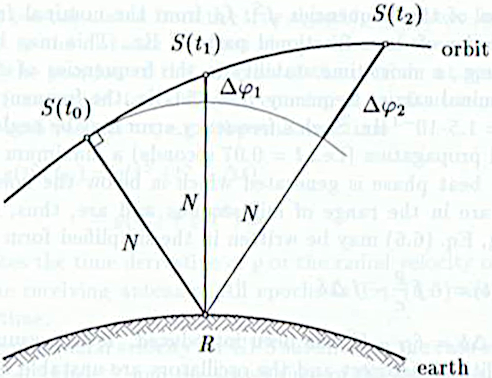
\includegraphics[width=\textwidth]{images/phasenverschiebung.jpg}
            \end{figure}
            \centering{\small[C,H-W,L]}
        \end{column}
    \end{columns}
\end{frame}

\begin{frame}{Zeitverzögerungen am Signal}
    S = Satellit, E = Empfänger
    \begin{align}
        t &= \text{Sende- /Empfangszeit} \\
        δ &= \text{zeitliche Verzögerungen, z.B. durch Rechenzeiten} \\
        t &= t(\text{GPS}) + δ
        \shortintertext{Zeitunterschied:}
        \increment t &= t_\text{E} - t^\text{S} = \increment t(\text{GPS}) +\incrementδ
        \shortintertext{Pseudoentfernung:}
        R &= \symup{c}\increment t = ρ + \symup{c}\incrementδ \label{eqn:pseudoentfernung}
        \shortintertext{Taylorreihe:}
        ρ\left(t_\text{E},\;t^\text{S}\right) &= ρ\left(t_\text{E},\;t^\text{S}+\increment t\right) = ρ\left(t^\text{S}\right)+\dot{ρ}\left(t^\text{S}\right)\cdot\increment t
        \shortintertext{Größe der ersten Korrektur:}
        \dot{ρ}\left(t^\text{S}\right)\cdot\increment t &\approx \SI{0.9}{\kilo\meter\per\second}\cdot\SI{0.07}{\second} =\SI{63}{\meter}
    \end{align}
\end{frame}

\begin{frame}{Ortskoordinaten}
    Man nimmt die Pseudoentfernung, Gleichung \eqref{eqn:pseudoentfernung}:
    \begin{align}
        R_\text{E}^\text{S}(t) &= ρ_\text{E}^\text{S}(t) + \symup{c}\incrementδ_\text{E}^\text{S}(t)
        \shortintertext{mit}
        ρ_\text{E}^\text{S}(t) &= \sqrt{\left(X^\text{S}(t)-X_\text{E}\right)^2+\left(Y^\text{S}(t)-Y_\text{E}\right)^2+\left(Z^\text{S}(t)-Z_\text{E}\right)^2}\;.
        \intertext{Der systematische Uhrenfehler wird angenähert}
        δ(t) &= a_0 + a_1(t-t_\text{r})+ a_2(t-t_\text{r})^2\;.
        \intertext{Es bleibt}
        R_\text{E}^\text{S}(t)& + \symup{c}δ^\text{S}(t) = ρ_\text{E}^\text{S}(t) + \symup{c}δ_\text{E}
    \end{align}
\end{frame}

\begin{frame}{Kreise}
        \begin{figure}
            \centering
            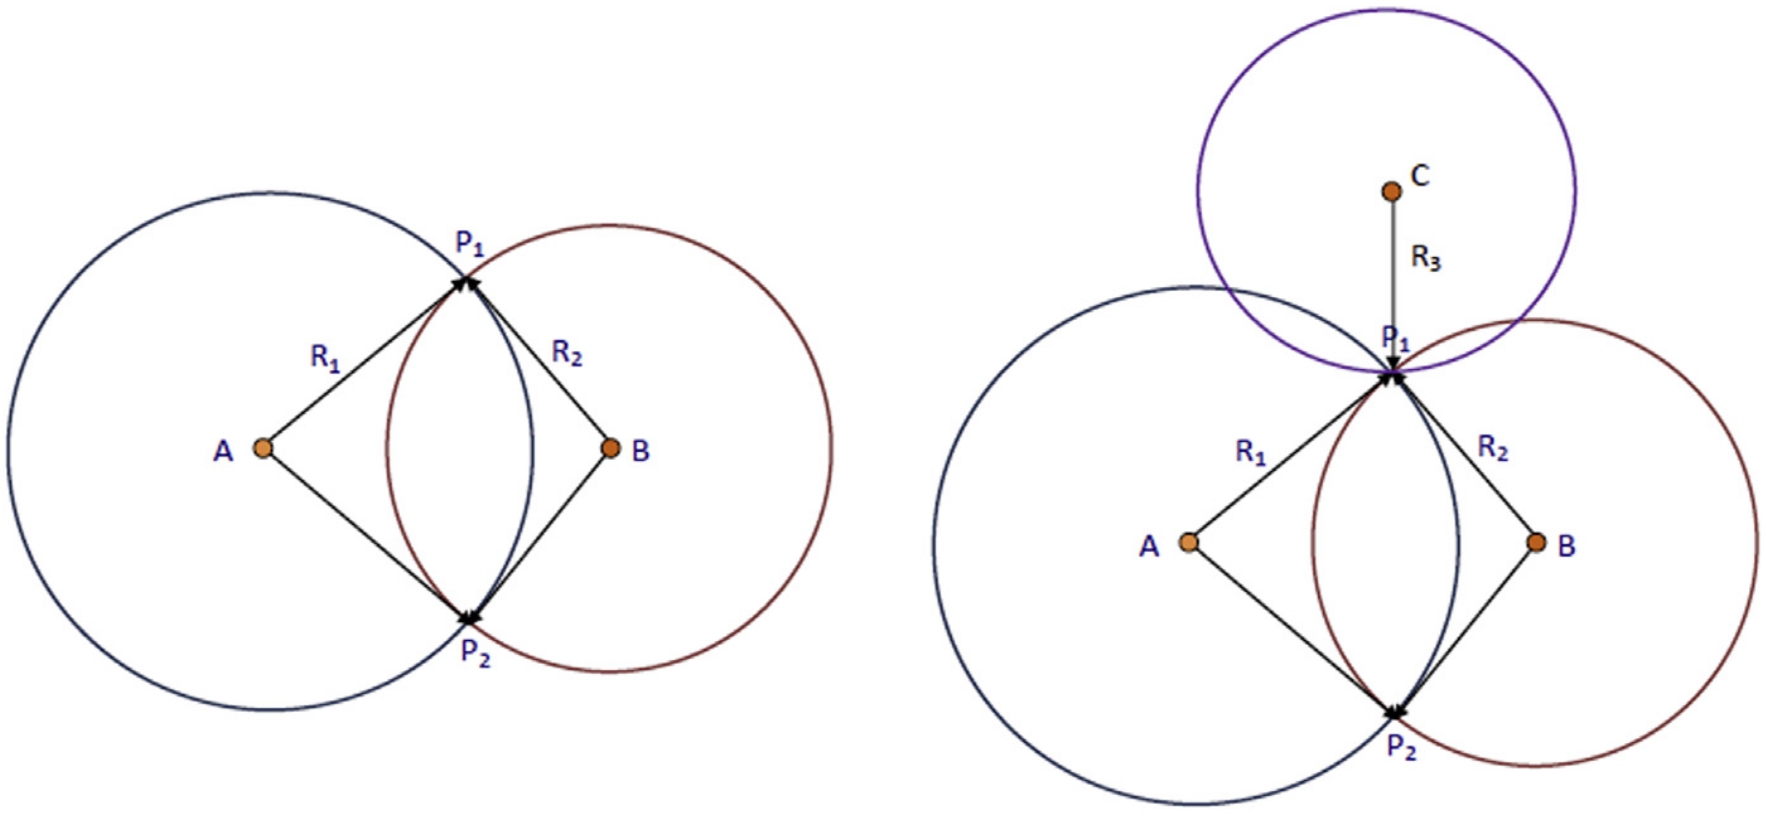
\includegraphics[width=\textwidth]{images/kreise-ort.png}
        \end{figure}
        \centering{\small [Acharya]}
\end{frame}

\begin{frame}{Atmosphärische Effekte}
    \begin{align}
        v_\text{ph} &= \lambda\cdot f \\
        v_\text{gr} &= v_\text{ph}-\lambda\frac{\symup{d}v_\text{ph}}{\symup{d}\lambda} \\
        v &= \frac{\symup{c}}{n} \\
        n_\text{ph} &= 1+\frac{c_2}{f^2}+\frac{c_3}{f^3}+\frac{c_4}{f^4}+\ldots \\
        n_\text{gr} &= 1-\frac{c_2}{f^2}+\ldots \\
    \end{align}
\end{frame}

\begin{frame}{Ionosphäre}
    \begin{columns}
        \begin{column}{0.5\textwidth}
            Fermat'sches Prinzip:
            \begin{align}
                s &= \int n\,\symup{d}\,s \\
                \increment^\text{Iono} &= \int n\,\symup{d}\,s-\int\symup{d}\,s_0 \\
                \increment^\text{Iono}_{gr} &= \SI{0.16}{\meter} \\
                \increment^\text{Iono}_{ph} &= \SI{-0.16}{\meter}
            \end{align}
        \end{column}
        \begin{column}{0.5\textwidth}
            Abhängigkeiten
            \begin{itemize}
                \item Sonnenstand
                \item Strecke durch die Ionosphäre
                \item Aktivität von Sonnenflecken
            \end{itemize}
        \end{column}
    \end{columns}
\end{frame}

\begin{frame}{Troposphäre}
    \begin{align}
        \increment^\text{Trop} &= \int(n-1)\symup{d}\,s \\
        N^\text{Trop} &= \num{e16}(n-1) \\
        \increment^\text{Trop} &= \num{e-16}\int N^\text{Trop}\symup{d}\,s \\
        N^\text{Trop} &= N^\text{Trop}_\text{trocken} + N^\text{Trop}_\text{nass} \propto \SI{90}{\percent} + \SI{10}{\percent} \\
        \increment^\text{Trop} &\approx \SI{2.3}{\meter}
    \end{align}
\end{frame}

\begin{frame}{Relativistische Effekte - Doppler Effekt}
    Für Satelliten
    \begin{align}
        \gamma &\approx 1+\num{9e-12}
        \intertext{Zeitdilatation}
        t &= \gamma\cdot\left(t'+\frac{v}{\symup{c}^2}x'\right)
        \intertext{Doppler Effekt 2. Ordnung}
        f &= \frac{f'}{\gamma}
    \end{align}
\end{frame}

\begin{frame}{Relative Uhren}
    Atomuhr im Satelliten: \\
    Grundfrequenz
    \begin{align}
        f_0 &= \SI{10.23}{\mega\hertz} \\
        \delta^\text{rel} &= \frac{f_0'-f_0}{f_0} = \frac{1}{2}\left(\frac{v}{\symup{c}}\right)^{\!\!2} + \frac{\mu}{\symup{c}^2}\left[\frac{1}{R_\text{E}+h}-\frac{1}{R_\text{E}}\right] = \num{-4.464e-10} \\
        \symup{d}f &= \num{4.464e-10}f_0 = \SI{4.57e-3}{\hertz}
    \end{align}
    Empfängeruhr:
    \begin{columns}
        \begin{column}{0.5\textwidth}
            \begin{align}
                v &\approx \SI{0.5}{\kilo\meter\per\second} \\
                \symup{d}f&\propto\num{e-12}f_0
            \end{align}
        \end{column}
        \begin{column}{0.5\textwidth}
            \centering
            Nach $\SI{3}{\hour}\!: \SI{10}{\nano\second}$ \\
            Fehler: $\SI{30}{\centi\meter}$ \\
        \end{column}
    \end{columns}
\end{frame}

\begin{frame}{Fehlerquellen}
    \begin{table}
        \centering
        \begin{tabular}{c c}
            \toprule
            {Fehlerquelle} & {Effekt} \\
            \midrule
            Signal    & Reflektionen in Atmosphäre und an Gebäuden \\
            Satellit  & falsche Orbitale \\
                      & Systematische Uhrfehler \\
            Empfänger & $^{\---}"^{\---}$ \\
                      & variable Emfängerfrequenz \\
            \bottomrule
        \end{tabular}
    \end{table}
\end{frame}
